\documentclass[newpage]{homework}
\newcommand{\hwname}{Zooey Nguyen}
\newcommand{\hwemail}{zooeyn@ucla.edu}
\newcommand{\hwclass}{CS 146}
\newcommand{\hwtype}{Homework}
\newcommand{\hwnum}{7}
\begin{document}
\maketitle


\question

\textbf{Base case:} The problem gives us the base case for dimension M=1. $S$ is the covariance matrix with one entry which is the variance of the feature $x$. The single eigenvalue of this matrix is simply the variance of the feature $x$ as it satisfies $Sx = \lambda x$.

\textbf{Induction step:} Suppose we have that the vectors $u_1, u_2, ..., u_M$ are the solutions to the maximisation problem in M-space and are the unit length orthogonal eigenvectors corresponding to the largest M eigenvalues of the MxM matrix $S_M$. We wish to find the next basis vector $u_{M+1}$.

Constraint 1: The new vector must be orthogonal to the previous vectors.
\begin{align*}
    0	&=  \sum_{i=1}^M    u_i^T u_{M+1}   \\
    0	&=  \sum_{i=1}^M    \alpha_i u_i^T u_{M+1}   \\
\end{align*}

Constraint 2: The new vector is of unit length.
\begin{align*}
    0	&=	u_{M+1}^T u_{M+1} - 1	\\
    0	&=	\beta (u_{M+1}^T u_{M+1} - 1)	\\
\end{align*}

Define the Lagrangian that we want to maximise, which is the variance of all the data projected onto the M+1 axis plus our multiplier quantities.
\begin{align*}
    L	&=	\frac{1}{M} \sum_n  (x_n \vdot u_{M+1})^2
         -  \sum_i        \alpha_i u_i^T u_{M+1}
         -  \beta (u_{M+1}^T u_{M+1} - 1)   \\
    L	&=	\frac{1}{M} (x_n u_{M+1})^T (x_n u_{M+1})
         -  \sum_i        \alpha_i u_i^T u_{M+1}
         -  \beta (u_{M+1}^T u_{M+1} - 1)   \\
    L	&=	u_{M+1}^T S u_{M+1}
         -  \sum_i        \alpha_i u_i^T u_{M+1}
         -  \beta (u_{M+1}^T u_{M+1} - 1)   \\
\end{align*}

Now take the derivative with respect to $u_{M+1}, \alpha_i, \beta$.
\begin{align*}
    \dv{L}{u_{M+1}}	&=	2Su_{M+1} - 2 \sum_i \alpha_i I u_{M+1} - 2\beta Iu_{M+1}	\\
    \dv{L}{u_{M+1}}	&=	2(S - (\sum_i \alpha_i + \beta)I)u_{M+1}   \\
    \dv{L}{\alpha_i}    &=  - \sum_i u_i^T u_{M+1}    \\
    \dv{L}{\beta}   &=  1 - u_{M+1}^T u_{M+1}
\end{align*}

Set all derivatives to zero and get some equations.
\begin{align*}
    0   &=  1 - u_{M+1}^T u_{M+1}   \\
    1   &=  u_{M+1}^T u_{M+1}   &\text{$u_{M+1}$ is unit} \\
    0    &= \sum_i u_i^T u_{M+1}    &\text{$u_{M+1}$ is orthogonal} \\
    0	&=	2(S - (\sum_i \alpha_i + \beta)I)u_{M+1}   \\
    Su_{M+1}    &=	(\sum_i \alpha_i + \beta)Iu_{M+1}   \\
    Su_{M+1}    &=	(\sum_i \alpha_i + \beta)u_{M+1}   \\
    Su_{M+1}    &=	\lambda_{M+1} u_{M+1}   \\
\end{align*}

We get that $u_{M+1}$ is an eigenvector of the covariance matrix $S$. But what's its eigenvalue $\lambda_{M+1}$? Now we maximise the variance, left multiply both sides.
\begin{align*}
    \max_{u_{M+1}} u_{M+1}^T Su_{M+1}    &=	u_{M+1}^T \lambda u_{M+1}   \\
    \max_{u_{M+1}} u_{M+1}^T Su_{M+1}    &=	\lambda_{M+1} u_{M+1}^T u_{M+1}   \\
    \max_{u_{M+1}} u_{M+1}^T Su_{M+1}    &=	\lambda_{M+1} \\
\end{align*}

The maximal $u_{M+1}$, which we already know is an eigenvector with eigenvalue $\lambda$, is achieved when its eigenvalue $\lambda$ is maximised.


\question
Center data to get data matrix.
\begin{align*}
    \mu_1    &=	0	\\
    \mu_2    &=	0	\\
    \mu_3    &=	0	\\
    X   &=  \begin{pmatrix}
            2 & 2 & 0   \\
            0 & -2 & 2  \\
            -2 & 0 & 0  \\
            0 & 0 & -2  \\
            \end{pmatrix}   \\
\end{align*}

Get covariance matrix.
\begin{align*}
    S	&=	\frac{1}{N} X^T X	\\
    S   &=  \begin{pmatrix}
        2 & 1 & 0   \\
        1 & 2 & -1  \\
        0 & -1 & 2  \\
        \end{pmatrix}   \\
\end{align*}

Find largest two eigenvalues from the characteristic equation of S and solve for the largest two eigenvalues.
\begin{align*}
    \det{S} &=	\lVert \begin{pmatrix}
                2 - \lambda & 1 & 0     \\
                1 & 2 - \lambda & -1    \\
                0 & -1 & 2 - \lambda   \\
                \end{pmatrix} \rVert    \\
    0   &=  -\lambda^3 + 6\lambda^2 - 10\lambda + 4 \\
    \lambda_1   &=  2 + \sqrt{2}    \\
    \lambda_2   &=  2   \\ 
    \lambda_3   &=  2 - \sqrt{2}   \\
\end{align*}

First principal component.
\begin{align*}
    Sw_1	&=	\lambda_1 w_1	\\
    (S - \lambda_1 I) w_1 &=  0   \\
    0   &=  \begin{pmatrix}
            - \sqrt{2} & 1 & 0   \\
            1 & - \sqrt{2} & -1  \\
            0 & -1 & - \sqrt{2}  \\
            \end{pmatrix}
            \begin{pmatrix}
            a_1    \\
            b_1    \\
            c_1    \\
            \end{pmatrix}   \\
    0   &=  b - \sqrt{2} a  \\
        &=  a - \sqrt{2} b - c  \\
        &=  -b - \sqrt{2} c \\
    (a, b, c)   &=  \boxed{(1, \sqrt{2}, -1)}   \\
\end{align*}

Second principal component.
\begin{align*}
    Sw_2	&=	\lambda_2 w_2	\\
    (S - \lambda_2 I) w_2 &=  0   \\
    0   &=  \begin{pmatrix}
            0 & 1 & 0   \\
            1 & 0 & -1  \\
            0 & -1 & 0  \\
            \end{pmatrix}
            \begin{pmatrix}
            a_1    \\
            b_1    \\
            c_1    \\
            \end{pmatrix}   \\
    0   &=  b \\
        &=  a - c  \\
        &=  -b \\
    (a, b, c)   &=  \boxed{(1, 0, -1)}   \\
\end{align*}


\question

Plot of the 100 largest eigenvalues.
\begin{figure}[htbp]
    \centering
    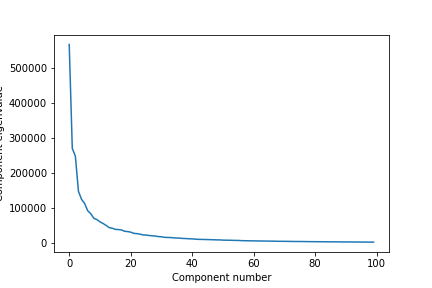
\includegraphics[width=0.6\textwidth]{3a.png}
\end{figure}

Plots of the four eigenvectors with highest eigenvalues. They each have only one nonzero value, corresponding to the pixel they represent.
\begin{figure}[htbp]
    \centering
    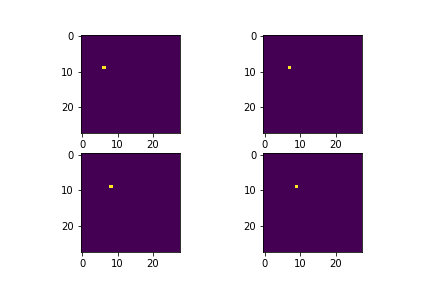
\includegraphics[width=0.8\textwidth]{3b.png}
\end{figure}

\newpage
Original image. 
\begin{figure}[htbp]
    \centering
    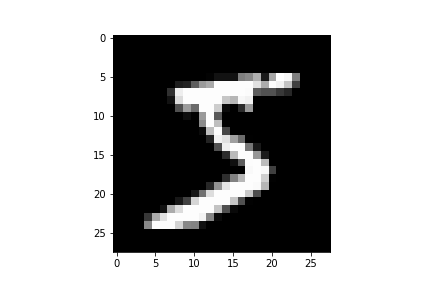
\includegraphics[width=0.3\textwidth]{3c-og.png}
\end{figure}

Plots of the compressed images. From left-right and top-down we have M = 1, 10, 50, 250, 784, and 0 dimensions. The quality increases as M increases. The basis vectors don't perfectly recover the original image but we get the clear shape of the number we are recovering. When M is 0, there are no eigen-pixels there to represent any of the image, so it's completely blank.
\begin{figure}[htbp]
    \centering
    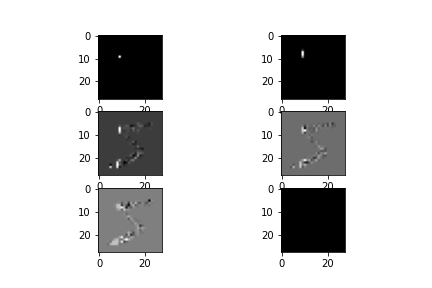
\includegraphics[width=\textwidth]{3c-compress.png}
\end{figure}


\question
Probability that ball 1 is never picked when we pick N times from a pile of N balls without replacement is zero. At some point you run out of balls so you have to have picked up ball 1.

Probability that ball 1 is never picked when we pick with replacement is $\left(\frac{N-1}{N}\right)^N$, which is definitely higher than zero.

For N = 1000 and limit to infinity.
\begin{align*}
    \left(\frac{1000-1}{1000}\right)^{1000}
    &=	(0.999)^{1000}	\\
    &=  0.36769542477   \\
    1/e &=  0.36787944117   \\
    A   &=  \lim_{N\to\infty} \left(\frac{N-1}{N}\right)^N  \\ 
    \ln A   &=\lim_{N\to\infty}  \ln \left(\frac{N-1}{N}\right)^N  \\ 
    \ln A   &=\lim_{N\to\infty}   \frac{\ln \left(\frac{N-1}{N}\right)}{1/N}   \\ 
    \ln A   &=\lim_{N\to\infty}   \frac{1/N(N-1)}{-1/N^2}   \\ 
    \ln A   &=\lim_{N\to\infty}   -\frac{N^2}{N^2-N}   \\ 
    \ln A   &=\lim_{N\to\infty}   -\frac{2N}{2N}   \\
    \ln A   &=  -1   \\
    A       &=  e^{-1}  \\
    A       &=  \frac{1}{e}
\end{align*}    


\question
Find $\pi_k$.
\begin{align*}
    L	&=	\sum_n \ln{\sum_j \pi_j P(x_n|\mu_j,\Sigma_j)}	+ \lambda(1 - \sum_j \pi_j) \\
    \dv{L}{\pi_k}   &=  \sum_n \frac{P(x_n|\mu_k,\Sigma_k)}{\sum_j \pi_j P(x_n|\mu_j,\Sigma_j)} - \lambda	\\
    \dv{L}{\lambda} &=  \sum_j \pi_j - 1    \\
    \pi_k \lambda &= \sum_n \frac{\pi_k P(x_n|\mu_k,\Sigma_k)}{\sum_j \pi_j P(x_n|\mu_j,\Sigma_j)}  \\
    \pi_k &= \frac{1}{\lambda} \sum_n \frac{\pi_k P(x_n|\mu_k,\Sigma_k)}{\sum_j \pi_j P(x_n|\mu_j,\Sigma_j)}    \\
    1   &=  \sum_j \pi_j    \\
    1   &=  \sum_j \frac{1}{\lambda} \sum_n \frac{\pi_k P(x_n|\mu_k,\Sigma_k)}{\sum_j \pi_j P(x_n|\mu_j,\Sigma_j)}  \\
    \frac{\lambda}{K}&=  \sum_n \frac{\pi_k P(x_n|\mu_k,\Sigma_k)}{\sum_j \pi_j P(x_n|\mu_j,\Sigma_j)}  \\
\end{align*}
???? don't know how to solve this one


\question
This dataset is not linear separable and we could not use a single layer to perfectly classify this set.
\begin{figure}[htbp]
    \centering
    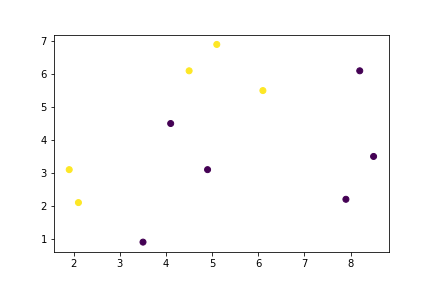
\includegraphics[width=\textwidth]{6a.png}
\end{figure}





\end{document}
